% UG project example file, February 2024
%
%   Added the "online" option for equal margins, February 2024 [Hiroshi Shimodaira, Iain Murray]
%   A minor change in citation, September 2023 [Hiroshi Shimodaira]
%
% Do not change the first two lines of code, except you may delete "logo," if causing problems.
% Understand any problems and seek approval before assuming it's ok to remove ugcheck.
\documentclass[logo,bsc,singlespacing,parskip,online]{infthesis}
\usepackage{ugcheck}


% Include any packages you need below, but don't include any that change the page
% layout or style of the dissertation. By including the ugcheck package above,
% you should catch most accidental changes of page layout though.

\usepackage[nopatch=footnote]{microtype} % recommended, but you can remove if it causes problems
\usepackage[round]{natbib} % recommended for citations
\usepackage{graphicx}
\usepackage{xcolor}
\usepackage{hyperref}

\begin{document}
\begin{preliminary}

\title{Extensions to libseff, an effect handler implementation using continuations in C}

\author{Jamie Day}

% CHOOSE YOUR DEGREE a):
% please leave just one of the following un-commented
%\course{Artificial Intelligence}
%\course{Artificial Intelligence and Computer Science}
%\course{Artificial Intelligence and Mathematics}
%\course{Artificial Intelligence and Software Engineering}
%\course{Cognitive Science}
%\course{Computer Science}
%\course{Computer Science and Management Science}
%\course{Computer Science and Mathematics}
%\course{Computer Science and Physics}
%\course{Software Engineering}
\course{Master of Informatics} % MInf students

% CHOOSE YOUR DEGREE b):
% please leave just one of the following un-commented
\project{MInf Project (Part 1) Report}  % 4th year MInf students
%\project{MInf Project (Part 2) Report}  % 5th year MInf students
%\project{4th Year Project Report}        % all other UG4 students


\date{\today}

\abstract{
\textit{libseff} is a lightweight effect handlers library for C using continuations. This paper investigates the existing performance of handler resolution and effect definition in this language, and implements and benchmarks new systems for each, which are found to increase the expressiveness of the language without affecting performance.
}

\maketitle

\newenvironment{ethics}
   {\begin{frontenv}{Research Ethics Approval}{\LARGE}}
   {\end{frontenv}\newpage}

\begin{ethics}

This project was planned in accordance with the Informatics Research
Ethics policy. It did not involve any aspects that required approval
from the Informatics Research Ethics committee.

\standarddeclaration
\end{ethics}


%\begin{acknowledgements}
%I would like to thank Saj's Shawarma and Grill, for always having my back through these hard times.
%\end{acknowledgements}


\tableofcontents
\end{preliminary}


\chapter{Introduction}

\section{Handlers' History and Usage}
Effect handlers are a control-flow paradigm that have been growing in popularity recently. \citep{effekt-paper} First invented as a programming construct at the University of Edinburgh, they have come into use by companies worldwide, including GitHub and Uber, and are used by tens of millions of developers worldwide through React's Hook implementation. \citep{impact_study}

While the first description of effect handlers in \citet{og-paper} was written in "a style that required
considerable mathematical sophistication to understand", \citep{impact_study} a later position paper by \citeauthor{action-position-paper} served to popularise the abstraction.

\section{What even are effect handlers?}
An \textit{effect} is an operation or group of operations that can be \textit{performed} to do some kind of action that cannot be done from local code. 

Effect handlers can be conceptualised in many ways. One way of thinking about effect handlers, and the lens through which the abstraction was originally invented in \cite{og-paper}, is as a generalisation of exception handlers - an exception handler that can return to the point the exception was raised is an effect handler. \citep{ocaml-paper}

Effect handlers can also be considered as calls to a function whose implementation depends on context, and which is not guaranteed to return. Which handler will handle the effect (and hence in this interpretation implement the function) depends on the context in which this block of code is running. \citep{award-paper}

\section{What is libseff?}

\textit{libseff} is an implementation of this idea in C. Differentiating \textit{libseff} from other implementations of effect handlers in C is its intended use by the general programming community, rather than specifically compiler writers, as is the case with languages such as \textit{libmpeff}. \citep{libseff_paper} \citep{libmprompt} \textit{libseff} is also designed to be as lightweight as possible to allow its use in embedded systems. \citep{libseff_paper}

\textit{libseff} at the time of writing has several peculiarities that make it unsuitable for use in production code in a large codebase. For example, the following code defines an effect: 
\begin{figure}[h]
    \centering
    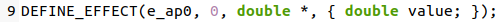
\includegraphics[width=0.9\linewidth]{eff_def.png}
    \caption{Taken from the ad.c test in the libseff repo}
\end{figure}

The leftmost argument to the macro is the name of the effect. The next argument is the ID of the effect, and this will be discussed below. The final arguments are the return value of the effect and a struct representing the parameters to the effect (all effects in \textit{libseff}, barring the return effect, must return a struct).

The ID is an integer that is used for the representation of effects - the PERFORM macro passes this value to the handler resolution function to find the relevant handler, for example. Requiring this to be predefined by the programmer is quite unusual and inconvenient - more on this in Chapter \ref{method}.

Another issue relating to the implementation of libseff is that only a maximum of 64 effects can be defined - again, more on this in \ref{method}.

These issues were solved - effect IDs are now autogenerated through being pointers to allocated memory, and libseff is now no longer limited in the number of effects it can represent.

These solutions were found to give negligible performance loss on most use cases.





\chapter{Context} \label{background}

\section{What are effect handlers?}
Effect handlers are a control flow mechanism that can be considered in several different ways: for example, as a generalisation of exception handlers. \citep{sep-log} The only difference is that exception handlers cannot return to the site where the exception was raised - effect handlers can. More specifically, effect handlers are passed a continuation, (often restricted in some way, such as delimitation \citep{old-paper}), that represents the code that requested the effect.

Such abstractions have many potential applications, including for backtracking, cooperative multi-threading and more \citep{effect_handlers_tutorial}. Real-world usage of this abstraction is already a reality, with use by Uber, Google, Facebook and more. \citep{impact_study}

Effect handler semantic systems have three parts:
\begin{itemize}
\item An \textit{effect signature}, which defines an effect
\item The instantiation of a \textit{handler}, which will handle the passed in coroutine
\item The site where the effect is performed
\end{itemize}

In Effekt \citep{effekt-paper} these three things look like this:

\begin{figure}[h]
    \centering
    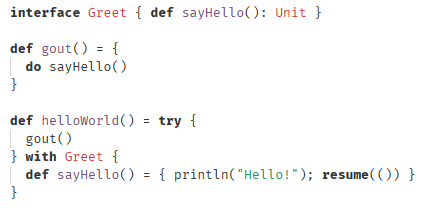
\includegraphics[width=0.5\linewidth]{basic_demo.png}
    \caption{Three parts of Effekt code showing the three different components of effect handlers. Adapted from \url{https://effekt-lang.org/quickstart}}
    \label{fig:basic}
\end{figure}

Let us expand from this basic example with something more involved:

\begin{figure}[h]
    \centering
    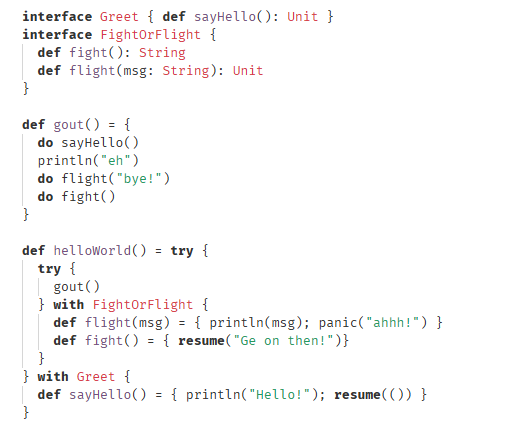
\includegraphics[width=0.9\linewidth]{effekt_2.png}
    \caption{More complex Effekt code}
    \label{fig:efkt2}
\end{figure}
\pagebreak
From this program we recieve the following output:

\begin{figure}[h]
    \centering
    
\includegraphics[width=0.5\linewidth]{effekt_2_out.png}
    \caption{Program output}
\end{figure}

This program displays several of the characteristic behaviours of effect handlers. First, note that effects will be handled in the closest (most recently wrapped) suitable handler - but that is not necessarily the closest handler. Further, the \textcolor{purple}{flight} operation is not required to return to the calling function; it is at the handler's discretion. Note also that data can be passed in and out of operation performances.


\section{Variants}
There are several different interpretations and implementations of effect handlers, with varying degrees of expressiveness and intuitiveness. Below are some of the more relevant divides.

\subsection{Lexical vs Dynamic binding}

Two methods for binding/scoping/resolving handlers are lexical and dynamic binding. Lexical binding has the advantage that handler resolution is a constant-time operation, but requires either a restrictive implementation or an expansive type system. As C barely possesses a type system at all, it was inevitable that libseff would use dynamic binding.

\subsection{Grouped vs Ungrouped Operations}

While in the ungrouped form effects are a single operation that is performed by itself, and a handler can handle many effects, with grouped operations an effect is a group of operations, and each handler can only handle one group. In this way effect definition looks more like interface definition in Java for example. libseff uses ungrouped effects (sometimes called singleton effects \citep{effekt-website}), which was judged to be more useful for the average programmer than the libmpeff implementation, which is grouped.

\subsection{Single vs Multishot continuations}

A handler that uses singleshot continuations can only resume a given continuation once, after which it will be overwritten by a new continuation or in some other way made invalid. Multishot continuations allow a given continuation to be resumed more than once, which is useful for tree searches and non-determinism for example. Given that the implementation of singleshot continuations is far simpler libseff uses those.

\subsection{Shallow vs Deep effect handlers}

A shallow effect handler binds an unhandled continuation when called, whereas a deep handler retains its binding over the continuation for subsequent calls. This is equivalent to saying that resumptions from a shallow handler do not return to that handler, whereas for deep handlers once a continuation has been wrapped in a handler it is always so. All shallow handlers can be turned into deep handlers by applying them recursively to continuations, although this can complicate type systems and be hard to reason about formally. libseff, and indeed most implementations, use deep handlers.

\section{What is libseff?}

Although much of the current usage of effect handlers is found in functional languages, there exist libraries that implement effect handling in almost every major language in which it is possible, including C. However, these libraries, such as \textbf{libmpeff}, are mostly designed specifically for compiler implementation, and as such offer features and make implementation decisions that do not necessarily make sense for the generic use case.\citep{libmprompt} \textbf{libseff}, on the other hand, is an implementation of effect handlers for C that is designed to be used directly by programmers.\citep{libseff_paper}








\chapter{Changes Made} \label{method}

\section{ID assignment}

Below we find the effect signature of an effect in libseff:

\begin{figure}[h]
    \centering
    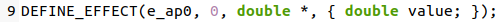
\includegraphics[width=0.9\linewidth]{eff_def.png}
    \caption{Taken from the ad.c test in the libseff repo}
\end{figure}

The leftmost argument to the macro is the name of the effect. The next argument is the ID of the effect, and this will be discussed below. The final arguments are the return value of the effect and a struct representing the parameters to the effect (all effects in \textit{libseff}, barring the return effect, must return a struct).

Note that the ID is an integer. This value must be provided by the programmer at compile time, and it must be unique - and it is the programmer's job to ensure this. This is not an ideal situation, as creating globally unique IDs is generally not an unsolved problem, and further this can be complicated to maintain; if two new code additions use the same ID, libseff will not give a compiler error. Indeed, if the handlers for these codebases never overlap, the code will run perfectly as intended - until a hapless programmer years down the line runs these two handlers one over the other and creates a truly insidious bug.

Note further that IDs must be unique with reference to any included libraries, including those that may not be available at compile time (dynamically linked libraries, also called shared libraries). This means that the IDs used by a specific library are not an implementation detail but instead part of the interface, and that libraries cannot refactor to define additional effects without either altering their public interface and making a breaking change, or over-allocating IDs, which causes particular problems with the other restriction in base libseff, discussed below.

A goal of this project was to have some method for assigning IDs automatically, with the following requirements:

\begin{itemize}
\item IDs must be unique: no two effects can have the same ID
\item The number of IDs able to be defined must not be bound in any meaningful way
\item Given the above constraints, checking whether a handler handles a given effect should be as fast as possible
\end{itemize}

We turn our attention to performing automatic ID generation. As noted%[CITE HERE]
, Universally Unique Identifiers (UUIDs) can be generated through the use of a so-called "magic pointer"%[CITE PLS]
, or a pointer to a fixed location in memory. Since pointers in C are guaranteed by the standard to only compare equal if they point to the same location%[CITE]
, (as perhaps you would expect), if a new memory address is assigned for each new effect, IDs generated this way are guaranteed to be unique. In this particular case, user-defined effect IDs are actually a pointer to the address that stores where the default generator for that effect is (it is a double pointer), because this is useful for fetching default handlers and there is no reason not to.

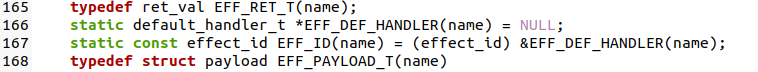
\includegraphics[scale=0.7]{ID_def_code.png}

One issue with this is that effect IDs are no longer fixed at compile time, which causes a few inefficiencies - for example, these effects can no longer be used in C's \textcolor{teal}{case} statements. Indeed, this cannot be avoided with any implementation that guarantees uniqueness without requiring knowledge of IDs chosen by included libraries, since dynamic libraries are only available at link time.

\section{Effect set representation}

Previously, effect sets were represented as a 64-bit integer, with each bit being 1 implying the handling of the effect with that index as an ID, and similarly 0 means its not handled, as shown below: 

\begin{figure}[h]
    \centering
    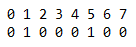
\includegraphics[width=0.3\linewidth]{effect_set.png}
    \caption{This 8-bit effect set handles effects 1 and 5, along with the return effect}
\end{figure}

This implementation was done to try to avoid a pointer dereference on determining whether a handler handles a given effect. The issues with a limit of 64 effects to large codebases do not need to be spelled out.

The current solution works more like a string - the effect set is a 0-terminated list of word-length integers, each corresponding to an effect. While this does add another layer of pointer indirection, it also allows the handling of any number of effects per handler, and importantly also implies that the total number of valid effect IDs is not limited to 64, as the previous implementation implied.

This is a valid representation because 0, the value of the null pointer, is guaranteed to never be allocated by C. Another special ID was also required - a signifier that this handler handles all effects. Although the address 0x1 is not guaranteed to be unallocated by the C standard, virtually every modern implementation of the C compiler allocates the first [X] bytes from 0 as an inacessible page, and it is thouroughly unlikely to be allocated to an effect halfway through a program.

0x1 is therefore used to signify two different things - when used as an effect ID and passed to libseff, the handler acquirer will understand that every handler handles this effect. When used in an effect set, libseff will understand the handler that handles this effect handles every effect - something that was trivial to write under the old system, bur requires special consideration now - we certainly cannot include every possible pointer in a list!

In the course of this process the default generator resolution process (what to do if there is no valid generator) was changed from an index into a length-64 array to a pointer allocation for each effect, retrievable through taking the value of the effect ID. Since it's a pointer anyway, it may as well point to the location of the pointer to the default generator.

\begin{figure}[h]
    \centering
    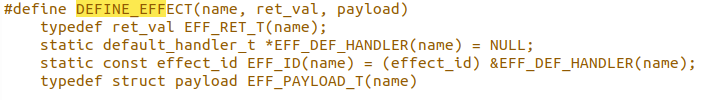
\includegraphics[width=1\linewidth]{defeff.png}
    \caption{Effect Definition}
    \label{fig:joooo}
\end{figure}

\section{Syntax changes}

These changes required changes to the syntax of the libseff library. Users now no longer have to (and can't) specify the ID of effects they define. More subtly, a common pattern seen even in the libseff code written to test and benchmark the library was for a handler to switch on the ID of an effect after being called - something no longer possible with effect IDs that aren't defined at compile time. These cases were rewritten as macros that inline to simply being if statements instead, which is less efficient for large switches but unlikely to come up in practise.

This syntax is slightly more unwieldy but ultimately the provided macros are simply syntactic sugar for unpacking the payload and do not need to be used for users to apply the full range of libseff.

\begin{figure}[h]
    \centering
    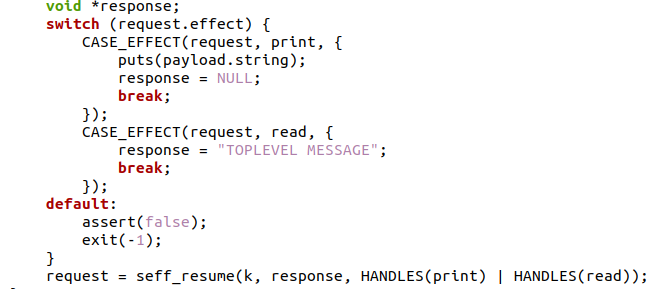
\includegraphics[width=1\linewidth]{oldswitch.png}
    \caption{The old switch implementation}
    \label{fig:oldswitch}
\end{figure}

\begin{figure}[h]
    \centering
    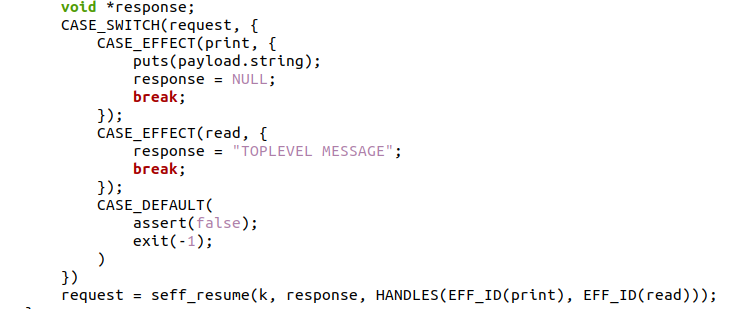
\includegraphics[width=1\linewidth]{newswitch.png}
    \caption{The new switch implementation with macros}
    \label{fig:newswitch}
\end{figure}







\chapter{Evaluation}

When evaluated against the benchmarks found in the \defcitealias{bench-joint}{joint effect benchmarking library}\citetalias{bench-joint}, it was found that this implementation ran faster than the original implementation on almost all benchmarks, which is an unexpected and slightly confusing, albeit welcome, result. 

\begin{figure}[h]
    \centering
    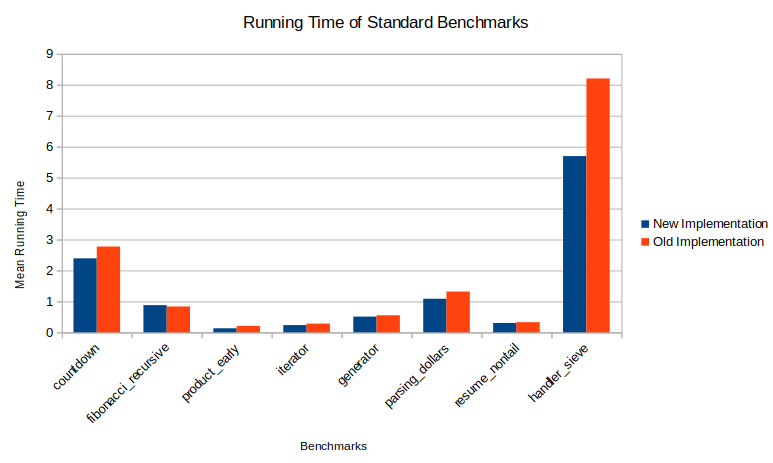
\includegraphics[width=1\linewidth]{bench_tests.PNG}
    \label{fig:benches}
\end{figure}








\chapter{Conclusion}

%In conclusion, my changes are awesome and should be merged into the main repo thank you sam :)

In conclusion, these changes increase the verbosity of the system at large and seem to lead to performance speedups as well. The objectives of solving these problems while keeping libseff fast and intuitive have been achieved.

% \bibliographystyle{plain}
\bibliographystyle{plainnat}
\bibliography{refs}

\nocite{*}


% You may delete everything from \appendix up to \end{document} if you don't need it.
\appendix

\chapter{Implemented Code}

The implementation of the changes discussed in this document can be found here: 
\url{https://github.com/Pendscraper/libseff_disc}


\end{document}
